\section{Notacja}

Przez $\mathbb{N}$ oznaczamy zbiór $\{0,1,2,\dots\}$, a przez $\mathbb{N}_+ = \{1,2,3,\dots\}$. 
Moc zbioru $A$ oznaczamy $|A|$. 
Logarytm naturalny z $x$ oznaczamy $\log(x)$. 
Dla $n\in\mathbb{N}_+$ przez $H_n=1+\frac{1}{2}+\cdots+\frac{1}{n}$ oznaczamy $n$-tą liczbę harmoniczną. 
Jeśli $f:\mathbb{R}\to\mathbb{R}$ jest funkcją to przez $f(\pm\infty)$ oznaczamy $\lim\limits_{x\to\pm\infty} f(x)$.

Niech $G=(V,E)$ będzie grafem prostym nieskierowanym. 
Przez $\mathrm{N}(v)=\{u\in V: \{u,v\}\in E\}$ oznaczamy zbiór sąsiadów dla $v\in V$. 
Odległość między $u$ i $v$ oznaczamy $\mathrm{d}(u,v)$ dla $u,v\in V$. 
Ekscentryczność $v\in V$ oznaczamy $\epsilon(v) = \max_{u\in V} \mathrm{d}(u,v)$. 

Jeśli $\mathbb{P}$ jest miarą prawdopodobieństwa na przestrzeni $\Omega$ to prawdopodobieństwo zdarzenia $A$ oznaczamy $\mathbb{P}[A]$. 
Dla zmiennej losowej $X:\Omega\to\mathbb{R}$ jej wartość oczekiwaną oznaczamy $\mathbb{E}[X]$ a jej wariancje $\mathrm{Var}[X]$. 
Funkcję masy prawdopodobieństwa (w skrócie PMF) oznaczamy $\mathbb{P}[X=t]$ a dystrybuante (w skrócie CDF) oznaczamy $F_X(t)=\mathbb{P}[X\le t]$ dla $t\in\mathbb{R}$. 
Mówimy, że zmienne losowe $X_1,\dots,X_n$ są IDD (independent and identically distributed) jeżeli są one niezależne oraz $F_{X_1}=\cdots=F_{X_n}$.


\section{Rodziny grafów}

W tej pracy ograniczymy rozważanie propagacji do konkretnych rodzin grafów.
Są to grafy ścieżkowe, gwiezdne, cykliczne oraz pełne.
Poniżej znajdują się szczegółowe definicje zbioru wierzchołków $V$ oraz zbioru krawędzi $E$ tych rodzin dla $n \in \mathbb{N}_+$.
Dodatkowo opisy te zawierają wizualizacje reprezentanta rodziny dla $n=5$.

\graphfamily{Graf ścieżkowy $\mathrm{P}_n$}
\[
    V = \{1, 2, \dots, n\}, \quad E = \{\{i, i+1\} : i \in \{1, 2, \dots, n-1\}\}.
\]
\begin{figure}[ht]
\begin{center}
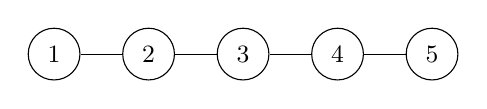
\begin{tikzpicture}[scale=1.2]
\foreach \i in {1,...,5} {
    \node[circle, draw, inner sep=4pt, minimum size=8pt] (v\i) at (\i, 0) {\small \i};
}
\foreach \i in {1,...,4} {
    \draw (v\i) -- (v\the\numexpr\i+1\relax);
}
\end{tikzpicture}
\caption{Graf $\mathrm{P}_5$}
\end{center}
\end{figure}

\graphfamily{Graf gwiazda $\mathrm{S}_n$}
\[
    V = \{0, 1, \dots, n\}, \quad E = \{\{0, i\} : i \in \{1, 2, \dots, n\}\}.
\]
\begin{figure}[ht]
\begin{center}
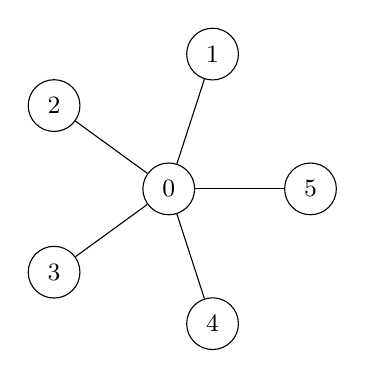
\begin{tikzpicture}[scale=1.2]
\node[circle, draw, inner sep=4pt, minimum size=8pt] (c) at (0,0) {\small 0};
\foreach \i in {1,...,5} {
    \node[circle, draw, inner sep=4pt, minimum size=8pt] (v\i) at (72*\i:1.5cm) {\small \i};
    \draw (c) -- (v\i);
}
\end{tikzpicture}
\caption{Graf $\mathrm{S}_5$}
\end{center}
\end{figure}

\graphfamily{Graf cykliczny $\mathrm{C}_n$}
\[
    V = \{1, 2, \dots, n\}, \quad E = \{\{i, i+1\} : i \in \{1, 2, \dots, n-1\}\} \cup \{\{n, 1\}\}.
\]
\begin{figure}[ht]
\begin{center}
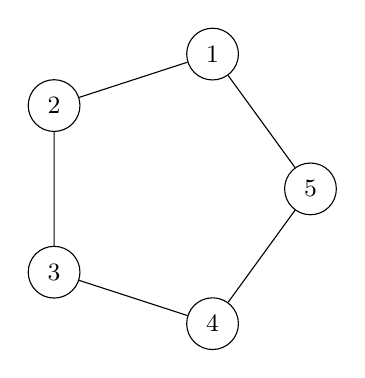
\begin{tikzpicture}[scale=1.2]
\foreach \i in {1,...,5} {
    \node[circle, draw, inner sep=4pt, minimum size=8pt] (v\i) at (72*\i:1.5cm) {\small \i};
}
\foreach \i in {1,...,4} {
    \draw (v\i) -- (v\the\numexpr\i+1\relax);
}
\draw (v5) -- (v1);
\end{tikzpicture}
\caption{Graf $\mathrm{C}_5$}
\end{center}
\end{figure}

\graphfamily{Graf pełny $\mathrm{K}_n$}
\[
    V = \{1, 2, \dots, n\}, \quad E = \{\{i, j\} : i, j \in \{1, 2, \dots, n\} \land i \ne j\}.
\]
\begin{figure}[ht]
\begin{center}
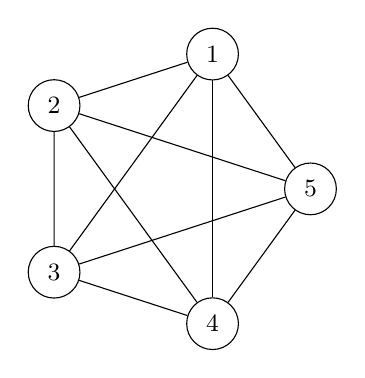
\begin{tikzpicture}[scale=1.2]
\foreach \i in {1,...,5} {
    \node[circle, draw, inner sep=4pt, minimum size=8pt] (v\i) at (72*\i:1.5cm) {\small \i};
}
\foreach \i in {1,...,5} {
    \foreach \j in {1,...,5} {
        \ifnum\i<\j
            \draw (v\i) -- (v\j);
        \fi
    }
}
\end{tikzpicture}
\caption{Graf $\mathrm{K}_5$}
\end{center}
\end{figure}


\section{Rozkłady prawdopodobieństwa}

Przedstawiamy specyfikacje klasycznych rozkładów prawdopodobieństwa obejmującą ich funkcje masy, wartości oczekiwane i wariancje. 

\distribution{Rozkład Bernoulliego $\mathrm{Ber}(p)$}
Próba Bernoulliego to doświadczenie losowe, którego wynik może być jednym z dwóch: sukces z prawdopodobieństwem $p \in (0;1)$ albo porażka z prawdopodobieństwem $1 - p$.
Zmienna losowa $X$ ma rozkład Bernoulliego jeżeli przyjmuje wartość $1$ w przypadku sukcesu i $0$ w przypadku porażki próby Bernoulliego.
Wtedy:
\[
\mathbb{P}[X = 0] = 1-p, \quad \mathbb{P}[X = 1] = p.
\]
Wartość oczekiwana i wariancja wynoszą:
\[
    \mathbb{E}[X] = p, \quad \mathrm{Var}[X] = p(1-p).
\]

\distribution{Rozkład dwumianowy $\mathrm{Bin}(n,p)$}
Zmienna losowa $X$ ma rozkład dwumianowy, jeżeli opisuję liczbę sukcesów w $n$ próbach Bernoulliego gdzie $n\in\mathbb{N}_+$, a każda próba ma prawdopodobieństwo sukcesu $p \in (0;1)$.  
Wtedy:
\[
\mathbb{P}[X = k] = \binom{n}{k}p^k{(1-p)}^{n-k}, \quad k \in \{0,1,\dots,n\}.
\]
Wartość oczekiwana i wariancja wynoszą:
\[
    \mathbb{E}[X] = np, \quad \mathrm{Var}[X] = np(1-p).
\]

\distribution{Rozkład geometryczny $\mathrm{Geo}(p)$}
Zmienna losowa $X$ ma rozkład geometryczny, jeżeli opisuje liczbę prób Bernoulliego potrzebnych do uzyskania pierwszego sukcesu gdzie każda próba ma prawdopodobieństwo sukcesu $p \in (0;1)$.  
Wtedy:
\[
    \mathbb{P}[X = k] = p{(1 - p)}^{k-1}, \quad k \in \mathbb{N}_+.
\]
Dystrybuanta jest równa:
\[
    \mathbb{P}[X\le t] = 1 - {(1-p)}^t.
\]
Wartość oczekiwana i wariancja wynoszą:
\[
    \mathbb{E}[X] = \frac{1}{p}, \quad \mathrm{Var}[X] = \frac{1 - p}{p^2}.
\]

\distribution{Rozkład ujemny dwumianowy $\mathrm{NegBin}(m, p)$}
Zmienna losowa $X$ ma rozkład ujemny dwumianowy, jeżeli opisuje liczbę prób Bernoulliego potrzebnych do uzyskania $m$ sukcesów gdzie $m\in\mathbb{N}_+$, a każda próba ma prawdopodobieństwo sukcesu $p \in (0;1)$.
Wtedy:
\[
\mathbb{P}[X = k] = \binom{k-1}{m-1} p^m {(1 - p)}^{k - m}, \quad k \ge m.
\]
Wartość oczekiwana i wariancja wynoszą:
\[
    \mathbb{E}[X] = \frac{m}{p}, \quad \mathrm{Var}[X] = \frac{m(1 - p)}{p^2}.
\]

\distribution{Rozkład normalny $\mathcal{N}(\mu, \sigma^2)$}
Zdefiniujmy funkcje
\[
    \varphi(t)=\frac{1}{\sqrt{2\pi}}e^{-\frac{t^2}{2}}, \quad \mathbf{\Phi}(t)=\int_{-\infty}^{t} \varphi(x)\;\mathrm{d}x.
\]
Niech $\mu \in \mathbb{R}$ oraz $\sigma > 0$. 
Zmienna losowa $X$ ma rozkład normalny, jeżeli jej funkcja gęstości wyraża się wzorem:
\[
    f_X(t) = \frac{1}{\sigma}\cdot\varphi\Big(\frac{t-\mu}{\sigma}\Big), \quad t \in \mathbb{R}.
\]
Dystrybuanta jest równa:
\[
    \mathbb{P}[X \le t] = \mathbf{\Phi}\Big(\frac{t-\mu}{\sigma}\Big), \quad t \in \mathbb{R}.
\]
Wartość oczekiwana i wariancja wynoszą:
\[
    \mathbb{E}[X] = \mu, \quad \mathrm{Var}[X] = \sigma^2.
\]
Jeśli $\mu = 0$ oraz $\sigma = 1$ to mówimy, że $X$ ma rozkład standardowy normalny.
$\varphi$ oraz $\mathbf{\Phi}$ są odpowiednio PDF jak i CDF takiego rozkładu.


\section{Fakty, sumy i nierówności}

W tej sekcji gromadzimy używane w pracy fakty pomocnicze, wzory sumacyjne oraz nierówności dotyczące zmiennych losowych i przekształceń analitycznych.

\begin{fact}\label{fact:max_CDF}
Niech $X_1,\dots, X_n$ będą IID zmiennymi losowymi o CDF równej $F_X$. 
Połóżmy \mbox{$Y = \max\{X_1,\dots, X_n\}$}. 
Wtedy 
\[
    F_Y(t)=F_X^n(t).
\]
\end{fact}

\begin{fact}\label{fact:min_CDF}
Niech $X_1,\dots, X_n$ będą IID zmiennymi losowymi o CDF równej $F_X$. 
Połóżmy \mbox{$Y = \min\{X_1,\dots, X_n\}$}. 
Wtedy 
\[
    F_Y(t)=1-{(1-F_X(t))}^n.
\]
\end{fact}

\begin{fact}\label{fact:sum_of_bin_RV}
Niech $X \sim \mathrm{Bin}(n,p)$ oraz $Y \sim \mathrm{Bin}(m,p)$ będą niezależnymi zmiennymi losowymi. 
Wtedy 
\[
    X + Y \sim \mathrm{Bin}(n+m, p).
\]
\end{fact}

\begin{fact}\label{fact:sum_of_bin_RV_2}
Niech $X \sim \mathrm{Bin}(n,p)$ oraz $Y \sim \mathrm{Bin}(m,r)$ będą niezależnymi zmiennymi losowymi.  
Połóżmy $Z=X+Y$.
Wtedy dla $k\in \{0,1,\ldots,n+m\}$ zachodzi
\[
    \mathbb{P}[X+Y=k] = \sum_{j=\max\{0,k-m\}}^{\min\{n,k\}} \binom{n}{j}\binom{m}{k-j}p^j{(1-p)}^{n-j}r^{k-j}{(1-r)}^{m-(k-j)}.
\]
\end{fact}

\begin{fact}\label{fact:pgf_bin}
Niech $X \sim \mathrm{Bin}(n, p)$.
Oznaczmy $q=1-p$.
Wtedy
\[
    \mathbb{E}[z^X]={(q+pz)}^n, \quad \mathbb{E}[Xz^X]=npz{(q+pz)}^{n-1}.
\]
\end{fact}

\begin{fact}\label{fact:sum_of_geo_RV}
Niech $X_1, \dots, X_m \sim \mathrm{Geo}(p)$ będą IID zmiennymi losowymi.
Wtedy 
\[
    X_1 +  \cdots + X_m \sim \mathrm{NegBin}(m, p).
\]
\end{fact}

\begin{fact}\label{fact:sum_of_normal_RV}
Niech $X \sim \mathcal{N}(\mu_1,\sigma_1^2)$ oraz $Y \sim \mathcal{N}(\mu_2,\sigma_2^2)$ będą niezależnymi zmiennymi losowymi. 
Wtedy 
\[
    X + Y \sim \mathcal{N}(\mu_1+\mu_2,\sigma_1^2+\sigma_2^2).
\]
\end{fact}


\begin{summ}\label{summ:binomial_0}
Niech $n\in\mathbb{N}$ oraz $x,y\in\mathbb{R}$. 
Wtedy
\[
    \sum_{k=0}^{n} \binom{n}{k} x^k y^{n-k}= {(x+y)}^n.
\]
\end{summ}

\begin{summ}\label{summ:binomial_1}
Niech $n\in\mathbb{N}$ oraz $x,y\in\mathbb{R}$. 
Wtedy
\[
    \sum_{k=0}^{n} k\cdot\binom{n}{k} x^k y^{n-k} = nx{(x+y)}^{n-1}.
\]
\end{summ}

\begin{summ}\label{summ:geo_0}
Niech $n\in\mathbb{N}$ oraz $x\in\mathbb{R}\setminus\{1\}$. 
Wtedy
\[
    \sum_{k=0}^{n} x^k=\frac{1-x^{n+1}}{1-x}.
\]
\end{summ}

\begin{summ}\label{summ:geo_1}
Niech $n\in\mathbb{N}$ oraz $x\in\mathbb{R}\setminus\{1\}$. 
Wtedy
\[
    \sum_{k=0}^{n} kx^k=\frac{x}{{(1-x)}^2}\cdot (nx^{n+1}-(n+1)x^n+1).
\]
\end{summ}

\begin{summ}\label{summ:geo_0_inf}
Niech $x\in(-1;1)$.
Wtedy
\[
    \sum_{k=0}^{\infty} x^k=\frac{1}{1-x}.
\]
\end{summ}

\begin{summ}\label{summ:geo_1_inf}
Niech $x\in(-1;1)$.
Wtedy
\[
    \sum_{k=0}^{\infty} kx^k=\frac{x}{{(1-x)}^2}.
\]
\end{summ}

\begin{summ}\label{summ:negbin_inf_0}
Niech $m\in\mathbb{N}$ oraz $x\in(-1;1)$.
Wtedy
\[
    \sum_{k=m}^{\infty} \binom{k-1}{m-1}x^k = \frac{x^m}{{(1-x)}^{m}}.
\]
\end{summ}

\begin{summ}\label{summ:negbin_inf_1}
Niech $m\in\mathbb{N}$ oraz $x\in(-1;1)$.
Wtedy
\[
    \sum_{k=m}^{\infty} k\cdot \binom{k-1}{m-1}x^k = \frac{mx^m}{{(1-x)}^{m+1}}.
\]
\end{summ}

\begin{inequality}\label{inequality:approximation_of_sum_by_an_integral}
Niech $a,b\in\mathbb{N}$, $a<b$ oraz $f:[a;b]\to\mathbb{R}$ będzie funkcją ciągłą i malejąca. 
Wtedy
\[
    \int_{a}^b f(x)\; \mathrm{d}x \le \sum_{k=a}^{b} f(k)\le f(a) + \int_{a}^b f(x)\; \mathrm{d}x.
\]
\end{inequality}

\begin{inequality}\label{inequality:harmonic_upper_bound}
Niech $n\in\mathbb{N}_+$. 
Wtedy
\[
    H_n \le 1 + \log(n).
\]
\end{inequality}

\begin{inequality}\label{inequality:log_vs_x}
Niech $x \in (0;1)$. 
Wtedy
\[
    \frac{1}{\log(\frac{1}{1-x})} \le \frac{1}{x}.
\]
\end{inequality}

\begin{inequality}[Nierówność między średnimi]\label{inequality:AM_GM}
Niech $x_1,x_2,\dots,x_n\ge 0$. 
Wtedy
\[
    \log(x_1\cdots x_n) \le n\cdot \log\left(\frac{x_1 + \cdots + x_n}{n}\right).
\]
Równość zachodzi wtedy i tylko wtedy gdy $x_1=\cdots=x_n$.
\end{inequality}

\begin{inequality}[Nierówność Markova]\label{inequality:Markov}
Niech $X$ będzie zmienną losową taką, że $X\ge 0$ oraz $\mathbb{E}[X]< \infty$. 
Wtedy dla dowolnego $t>0$
\[
    \mathbb{P}[X\ge t] \le \frac{\mathbb{E}[X]}{t}.
\]
\end{inequality}

\begin{inequality}[Nierówność Cauchy'ego-Schwarza]\label{inequality:Cauchy_Schwarz}
Niech $X,Y$ będą zmiennymi losowymi takimi, że $\mathbb{E}[X^2],\mathbb{E}[Y^2]< \infty$. 
Wtedy
\[
    \mathbb{E}[X\cdot Y] \le \sqrt{\mathbb{E}[X^2]}\cdot \sqrt{\mathbb{E}[Y^2]}.
\]
\end{inequality}

\begin{inequality}[Nierówność Jensena]\label{inequality:Jensen} 
Niech $n\in\mathbb{N}_+$ oraz \mbox{$g:\mathbb{R}^n\to\mathbb{R}$} będzie funkcją wypukłą, zaś $X_1,\dots, X_n$ będą zmiennymi losowymi (niekoniecznie niezależnymi). 
Wtedy
\[
    g(\mathbb{E}[X_1],\dots, \mathbb{E}[X_n]) \le \mathbb{E}[g(X_1,\dots,X_n)].
\]
W szczególności, ponieważ $\max$ jest funkcją wypukłą, mamy:
\[
    \max(\mathbb{E}[X_1],\dots, \mathbb{E}[X_n]) \le \mathbb{E}[\max(X_1,\dots,X_n)].
\]
\end{inequality}